\section{Challenges Of \spath Caching}\label{sec:competitors}

In this section we qualify the differences between static (no change in cache content at service runtime) and dynamic caching (Cache content is changed at service runtime) of \spathsns. We also introduce our state of the art competitor and explain why it is not an adequate solution for the \spath caching problem.


Using a dynamic cache\footnotemark and calculating the utility of each path is very expensive. If a dynamic cache is used, and we want to ensure it always keeps the most useful paths in the cache, it will be very expensive to calculate the utility of a new query with respect how much it overlaps with existing \spaths (i.e. how many vertices it shares with an existing \spathns) and how likely it will be able to answer a query in the future, thus adding a substantial overhead to query processing. As the utility of a \spath is so expensive to calculate, while the \spath service is running, it violates goal \ref{item:goal2} in section \ref{subsec:goals}.

Using \lru as the cache replacement policy in a dynamic cache ensures that only minimal overhead is added by using a dynamic cache. When a new query is submittet \lru evicts the least recently used \spath and keeps the most recently used \spaths in the cache.
\lru, however, has several shortcomings: 
\begin{itemize}
\item It has no way to determine the usefulness of inserting a path (i.e. no scoring function), which violates goal \ref{item:goal3} (Sec. \ref{subsec:goals}). 
\item Because \lru does not have a scoring function then, even if a path $P$ is valuable (covers many potential queries), if a sequence of consecutive queries, which $P$ can not cover, is submitted, then P will be evicted. 
\item \lru also does not have any way to optimize utilization of the cache space available, possibly wasting a lot of space. 
\end{itemize}

If no additional structure is added then querying the cache may require a scan of all paths in the cache to examine the cache can answer a query or not.

\footnotetext{Every time a new query is submitted we consider evicting an old item from the cache and inserting the new query, using a replacement policy e.g. \lru}





To give an example of \lrus shortcomings we assume a cache of size 10 (i.e. has space for 10 vertices), using \lruns, and running on the map from figure \ref{fig:rxmap}. The queries submittet to the system are: 
Q1:$Q_{1,6}$, Q2:$Q_{2,6}$, Q3:$Q_{1,4}$, Q4:$Q_{4,7}$, Q5:$Q_{1,5}$, Q6:$Q_{3,6}$.
The answer to Q1 and Q2 (Fig. \ref{fig:rxmap}A,B) are added to the cache as both results have a length of 5 and they can both fit. Q3 results in a cache hit with Q1, but when Q4 is submitted Q1 will be evicted and Q4:$\{v_4,v_5,v_7\}$ inserted. Q5, which \textit{could} have been answered by Q1, now results in the eviction of Q2 and insertion of Q5:$\{v_1,v_3,v_4,v_5\}$. Q6 is not covered by Q3 or Q5 so it results in a cache miss, and because there are 7 nodes in the cache and Q6:$\{v_3,v_4,v_5,v_6\}$ has 4 nodes, then Q3 will be evicted (since it was inserted first) and Q6 inserted. 
The end result is that 30\% of the cache space is wasted and out of the 6 queries only we only resulted in a 1 cache hit, we could have had 3 if we kept Q1 in the cache.




% ---
% more beneficial to fill the cache offline and use a static cache, i.e. not evicting or inserting \spaths while the system is running.
% ----

% Intro to section; Why do we have baseline competitors, which ones will be introduced, and why those? 

% \lru is a competitor, but can not achieve good performance because:
% \begin{itemize}	
% 	\item Has no way to determine the usefulness of adding a path (i.e. no scoring function)
% 	\item Even if a path P is good (covers many queries), then if a sequence of consecutive queries comes which P can not cover, then it will be evicted.
% 	\item Has no way to optimize the number of paths in the cache, so available cache space may go unused.
% 	\item 
% \end{itemize}






\section{Contribution} \label{sec:contribution}

Intro to section \\
Show benefits of a static cache over a dynamic cache.\\
List all advantages of a static cache solution \\
(\textit{Static cache} solves goal 2. has zero maintenance cost after filling the cache.)

explain what will be introduced, which sub-problems are considered, and which subsections presents what.


\begin{table}
\begin{tabular*}{\columnwidth}{|l||p{0.78\columnwidth}|}
\hline
\bf Symbol		& \bf Meaning \\\hline
$Q_{s,t}$		& \spath query from $s$ to $t$ \\\hline
$SP_{s,t}$		& \spath from $s$ to $t$ \\\hline
$\zeta$ 		& The Cache \\\hline
$\zeta_i$		& i'th item in the cache \\\hline
$\chi_{s,t}$		& Calculates the frequency of a (sub-)path \\\hline
$\Phi(sp)$		& Finds the set of all sub-paths in a \spath $sp$ \\\hline
$\gamma$		& The set of all unique (sub-)paths in $\zeta$ \\\hline
$\tau$			& Calculates the total utility of the content in the cache \\\hline 
\end{tabular*}
\caption{Table of Symbols}
\label{tab:symbols}
\end{table}


\begin{figure}[bht]
  \center
        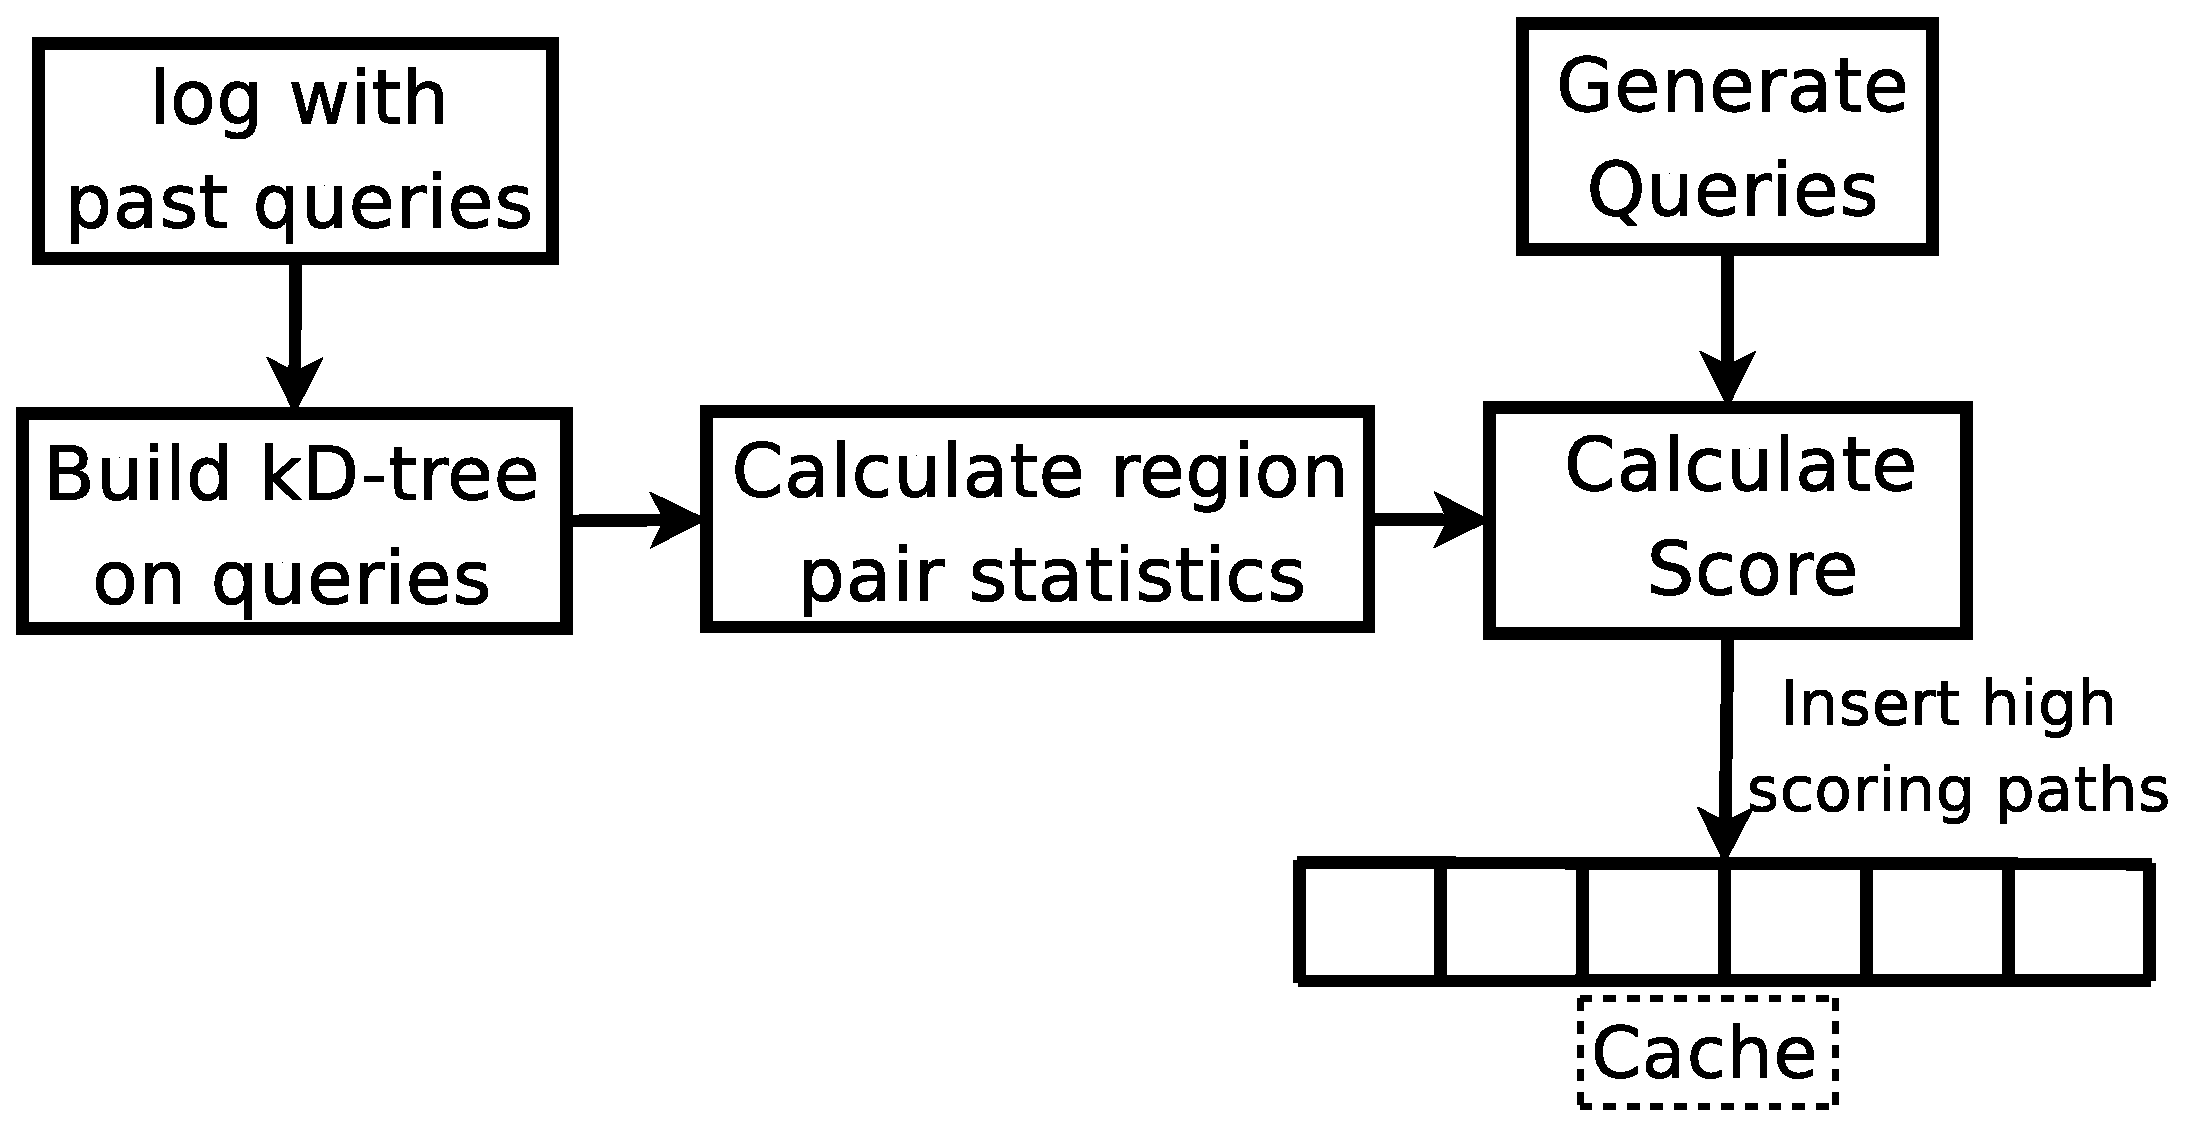
\includegraphics[width=0.5\textwidth]{figures/fillcache}
        \caption{Insertion of cache elements in offline phase.}
  \label{fig:fillcache}
\end{figure}


\subsection{Benefit model}

We will define our goals more formally, introducing the benefit equations we aim to minimize.

A query is a pair of vertice ids $(v_s, v_t)$, denoted $Q_{s,t}$ and the \spath returned from such query we denote $SP_{s,t}$. 
In order to evaluate goal \ref{item:goal3} we calculate the utility of the content in the cache, denoted $\tau$. To calculate $\tau$ we find the set of unique sub-paths from all \spaths in the cache ($\zeta$) and sum up the frequency, $\chi_{s,t}$, of each unique sub-path.

In order to evaluate our method we try to maximize $\tau$ (Eq. \ref{eq:benifit}).



\begin{equation} \label{eq:gamma}
 \gamma = \bigcup\limits_{\forall \spath \in \zeta} \Phi(\spath) \\
\end{equation}
\begin{equation} \label{eq:benifit}.
\tau = \sum\limits_{\forall SP_{s,t} \in \gamma} \chi_{s,t}
\end{equation}


\begin{table}
\begin{tabular}{l l p{0.78\columnwidth}}
Q1:	&	$Q_{1,6} =$ 	& $\{v_1,v_3,v_4,v_5,v_6\}$\\
Q2:	&	$Q_{2,6} =$ 	& $\{v_2,v_3,v_4,v_5,v_6\}$ \\
Q3:	&	$Q_{1,4} =$ 	& $\{v_1,v_3,v_4\}$ \\
Q4:	&	$Q_{4,7} =$ 	& $\{v_4,v_5,v_7\}$ \\
Q5:	&	$Q_{1,5} =$ 	& $\{v_1,v_3,v_4,v_5\}$ \\
Q6:	&	$Q_{3,6} =$ 	& $\{v_3,v_4,v_5,v_6\}$ \\
\end{tabular}
\caption{Example Queries}
\label{tab:queries}
\end{table}

\begin{table}
\begin{tabular}{r p{0.78\columnwidth}}
$\Phi(SP_{1,6})=$ 	& $\{SP_{1,3},SP_{1,4},SP_{1,5},SP_{1,6},SP_{3,4},SP_{3,5},$\\
		 	& $SP_{3,6},SP_{4,5},SP_{4,6},SP_{5,6}\}$ \\
$\Phi(SP_{2,6})=$ 	& $\{SP_{2,3},SP_{2,4},SP_{2,5},SP_{2,6},SP_{3,4},SP_{3,5},$ \\
			& $SP_{3,6},SP_{4,5},SP_{4,6},SP_{5,6}\}$ \\
$\Phi(SP_{1,4})=$ 	& $\{SP_{1,3},SP_{1,4},SP_{3,4}\}$ \\
$\Phi(SP_{4,7})=$ 	& $\{SP_{4,5},SP_{4,7},SP_{5,7}\}$ \\
$\Phi(SP_{1,5})=$ 	& $\{SP_{1,3},SP_{1,4},SP_{1,5},SP_{3,4},SP_{3,5},SP_{4,5}\}$ \\
$\Phi(SP_{3,6})=$ 	& $\{SP_{3,4},SP_{3,5},SP_{3,6},SP_{4,5},SP_{4,6},SP_{5,6}\}$ \\\hline
$\gamma =$ 		& $\{SP_{1,3},SP_{1,4},SP_{1,5},SP_{1,6},SP_{3,4},SP_{3,5},$ \\
			& $SP_{3,6},SP_{4,5},SP_{4,6},SP_{5,6},SP_{2,3},SP_{2,4},SP_{2,5},$ \\
			& $SP_{2,6},SP_{4,5},SP_{4,7},SP_{5,7}\}$  \\
\end{tabular}
\caption{$\Phi$ results for queries in table \ref{tab:queries}}
\label{tab:phi}
\end{table}

When we want to evaluate the utility of $\zeta$ we first calculate $\gamma$ for each \spath. Table \ref{tab:phi} shows the set of sub-paths from the \spaths for each query Q1-Q6 from table \ref{tab:queries}. Once we have all the sets of sub-paths from the cache content, we use equation \ref{eq:gamma} to union them together and obtain the set of unique sub-paths in the cache, $\gamma$ (see table \ref{tab:phi}). After we have obtained $\gamma$, we use equation \ref{eq:benifit} to calculate the total benifit we expect to have with the content in $\zeta$.

\subsection{Hardness Analysis}
Theoretical analysis showing how hard the problem is to solve for \spath caching.\\
show it is NP-Hard
 

\subsection{Greedy algorithm}
shows in more detail how we propose to solve our problem


\subsection{Statistics extraction}

\subsubsection{Partition map} 
solves goal 1. reduce time on \spath calculation as it aids the cache with information on which paths may be useful.\\ 
discussion of kD-Tree.


\subsection{Cache representations and cache concepts} 

\subsubsection{Simple array of paths} - baseline for goal 2, unoptimized and expensive to use.

\subsubsection{Simple array of paths inverted list} - solves goal 2, reduces the query time of the cache.

\subsubsection{Graph representation} - solves goal 1, allows for more paths in cache, which should translate more cache hits.

\subsubsection{Sharing subpaths} - solves goal 1, allows for more paths in cache, translating to more cachehits. Unfortunately has a negative impact on goal 2 as it introduces some overhead in query time.

